\documentclass[10pt]{scrartcl}

\usepackage[utf8]{inputenc}
\usepackage{tabularx}
\usepackage{longtable}
\usepackage[ngerman]{babel}
\usepackage[automark]{scrpage2}
\usepackage{amsmath,amssymb,amstext}
%\usepackage{mathtools}
\usepackage[]{color}
\usepackage[]{enumerate}
\usepackage{graphicx}
\usepackage{lastpage}
\usepackage[perpage,para,symbol*]{footmisc}
\usepackage{listings} 
\usepackage[pdfborder={0 0 0},colorlinks=false]{hyperref}
\usepackage[numbers,square]{natbib}
\usepackage{color}
\usepackage{colortbl}
\usepackage[absolute]{textpos}
\usepackage{float}
\usepackage[colorinlistoftodos,textsize=small,textwidth=2cm,shadow,bordercolor=black,backgroundcolor={red!100!green!33},linecolor=black]{todonotes}

\lstset{numbers=left, numberstyle=\tiny, numbersep=5pt, breaklines=true, showstringspaces=false} 
\restylefloat{figure}

%changehere
\def\titletext{Lab 1 : MANET}
\def\titletextshort{Praktikum 1}
\author{André Harms, Oliver Steenbuck}

\title{\titletext}

%changehere Datum der Übung
\date{09.11.2011}

\pagestyle{scrheadings}
%changehere
\ihead{TT1, Schmidt}
\ifoot{Generiert am:\\ \today}

\cfoot{Oliver Steenbuck, André Harms}


\ohead[]{\titletextshort}
\ofoot[]{{\thepage} / \pageref{LastPage}}

\setlength{\parindent}{0.0in}
\setlength{\parskip}{0.1in}

\begin{document}
\maketitle

\setcounter{tocdepth}{3}
\tableofcontents

	\listoftables                                 												% 
	\listoffigures   

\section{Testaufbau}
	Die vier im Test verwendeten Router (APs) (110, 210, 104, 204) wurden wir in Abbildung \ref{img:testAufbau} gezeigt angeordnet. 	Von allen Access Points wurden die Antennen entfernt um reale Umgebungsbedingungen im Labor zu simulieren und den Aufbau eines Mesh-Netzwerkes zu ermöglichen. Beispielhaft sind in den Listings \ref{code_110_babel} und \ref{code_110_olsr} die Konfiguration des Babel bzw. OLSR Daemons für den Router 110 dargestellt, mit Ausnahme der entsprechend geänderten Adressen wurden alle Router identisch konfiguriert.  
		Alle Messungen wurden mit JPerf zwischen an den Routern 204 und 110 angeschlossenen Workstations durchgeführt, die Anzahl der Hops die zwischen den Messpunkten wurden mit Tracert, bzw. über die Weboberfläche des OLSR Daemons festgestellt. Ziel des Versuchsaufbaus war es das Mesh-Netzwerk so aufzubauen das Messungen über alle 4 Router hinweg durchgeführt werden können.
		
	\begin{figure}[H]
        \centering
                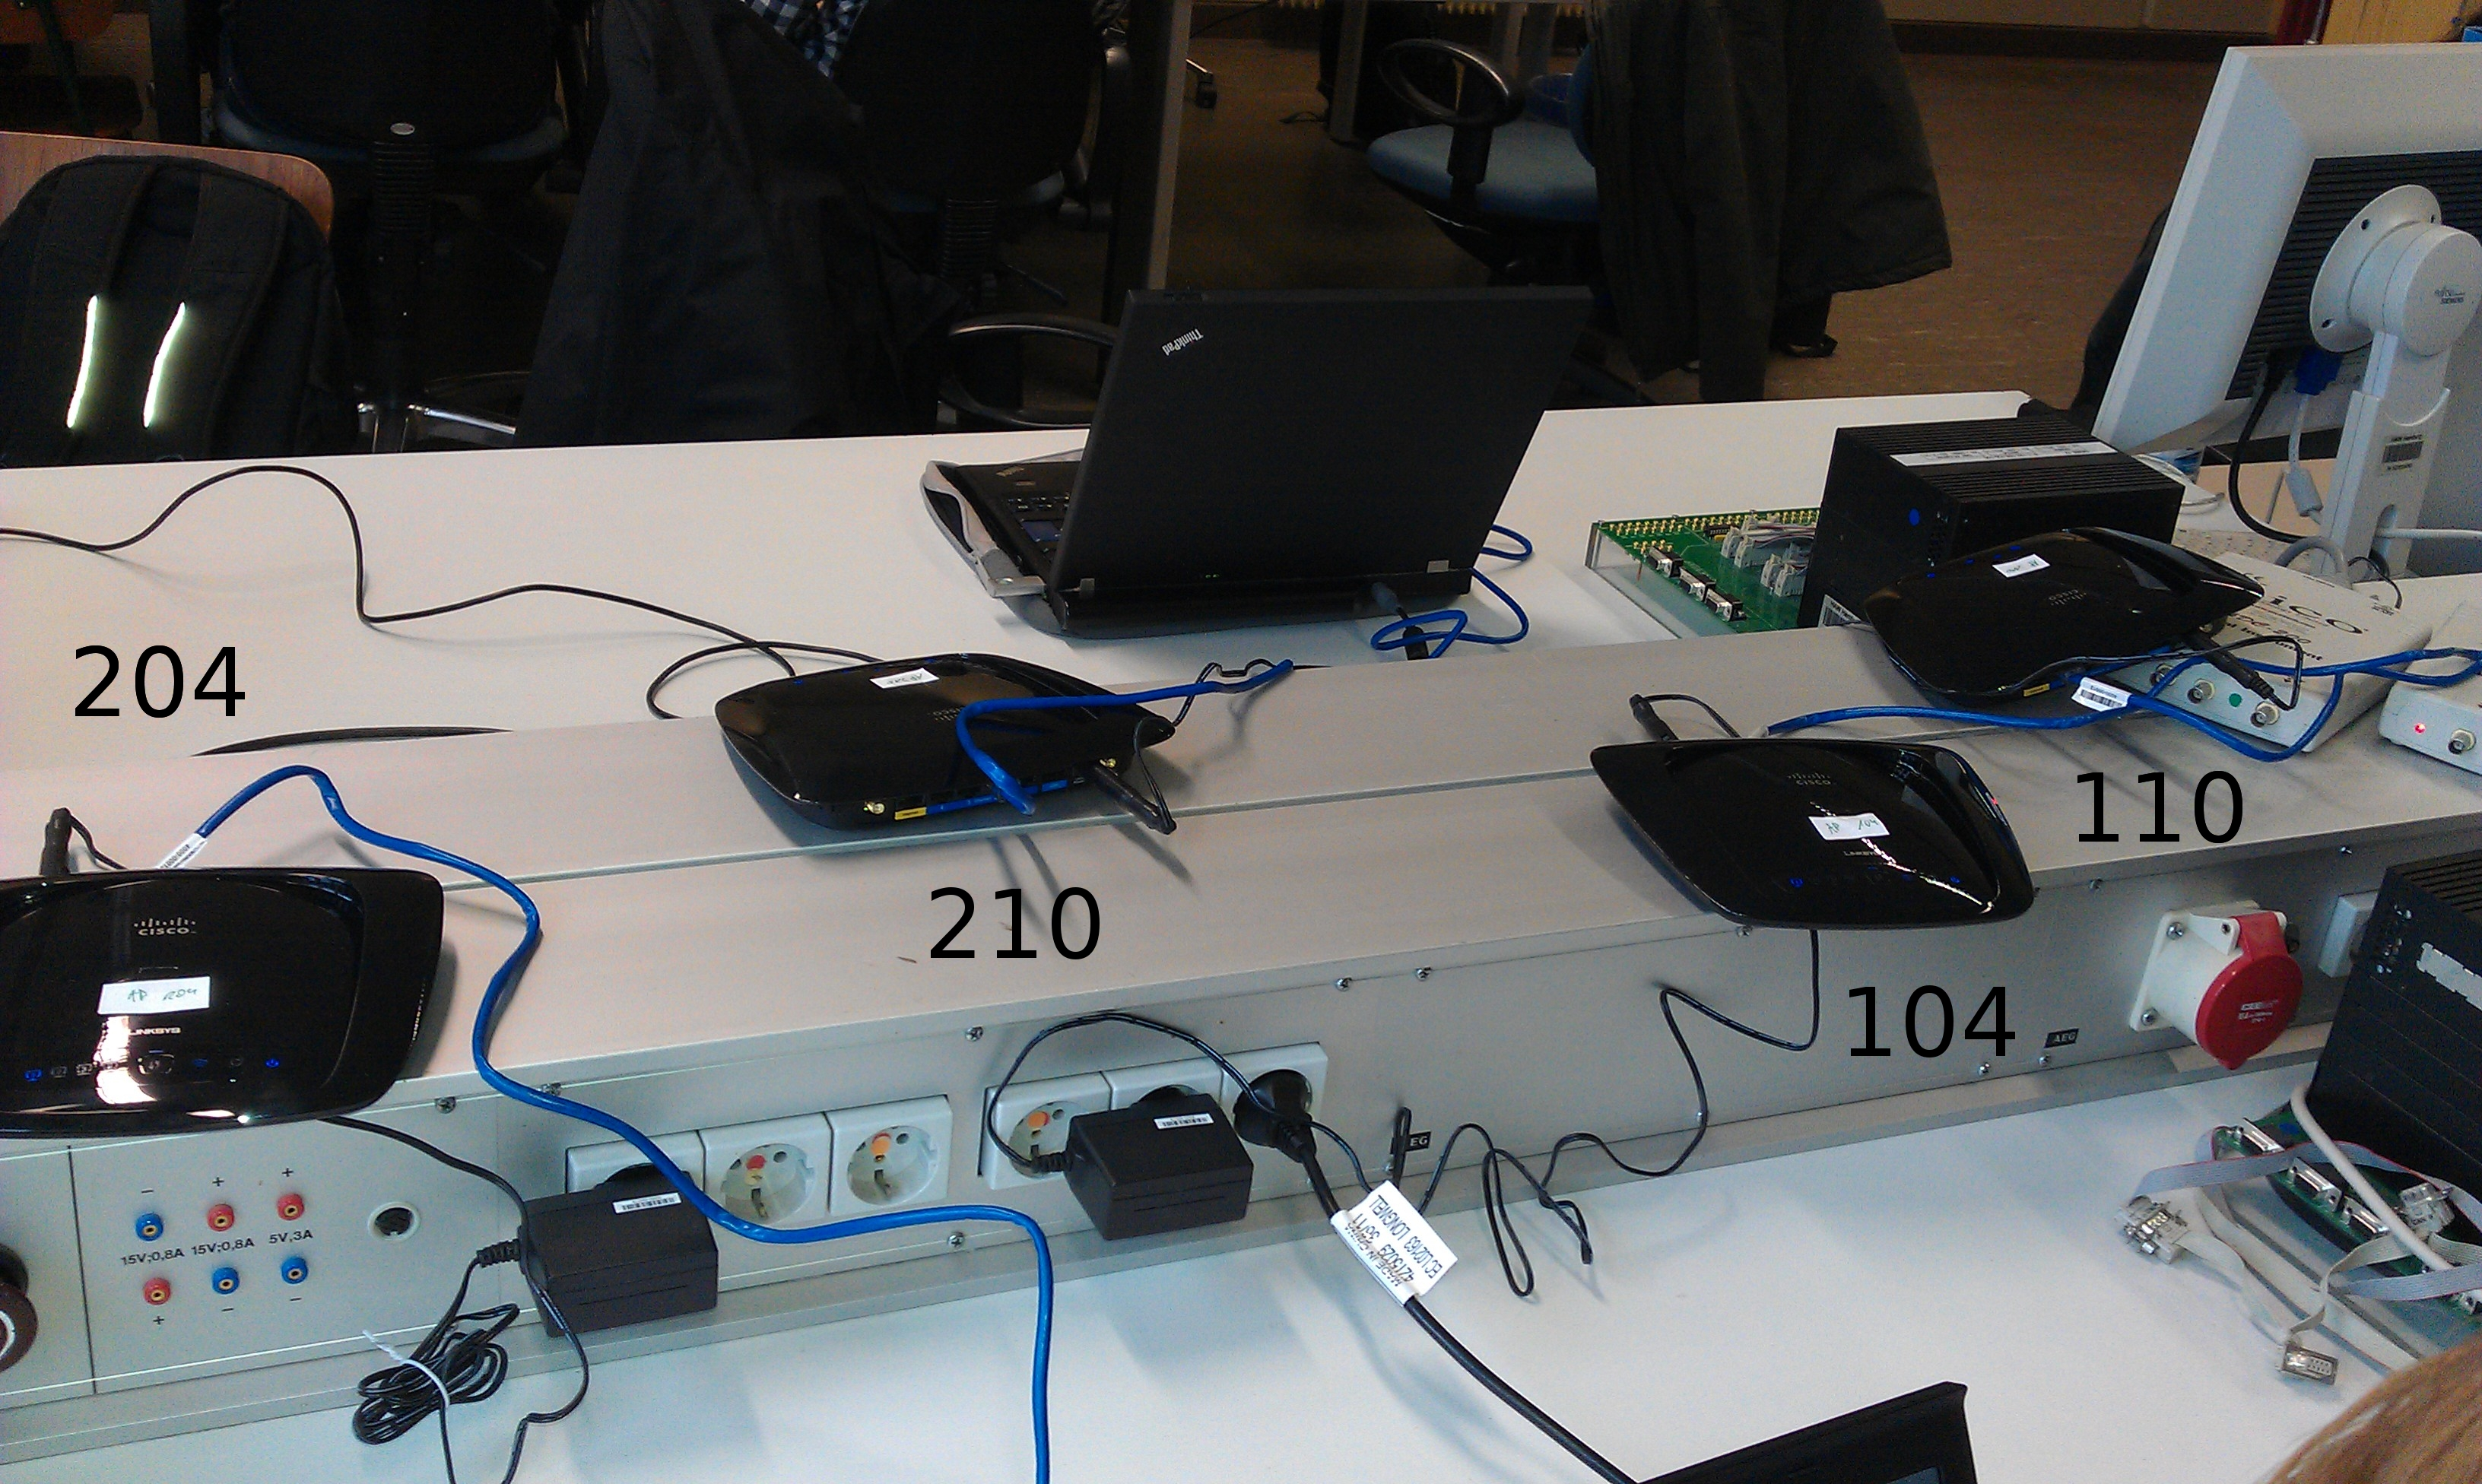
\includegraphics[width=\textwidth]{img/AufbauBild}
        \caption{Physikalische Anordnung Router}
        \label{img:testAufbau}
	\end{figure}	
	
	
	\lstinputlisting[label=code_110_babel,caption=Babel Konfiguration: Router 110, frame=single, language=bash]{../Startscripte/110/babeld_start.sh}	
	\lstinputlisting[label=code_110_olsr,caption=OLSR Konfiguration: Router 110, frame=single, language=bash]{../Startscripte/110/olsrd_start.sh}	
	
	
\section{Routing Protokolle}
	Im folgenden werden die beiden genutzen Routing Protokolle Babel und OLSR kurz erläutert und verglichen.
	
	\subsection{Babel}
	Babel ist ein Distance-vector Protokoll funktioniert also ähnlich wie RIP oder IGRP über das Versenden von kürzesten Wegen an andere Router. Distance-vector Protkolle funktionieren in der Regel mit einer Variante des hier dargestellten Algorithmus.
	
	\begin{enumerate}
		\item Routingtabelle erstellen
		\item \label{dvp:ueber} Routingtabelle an benachbarte Router übermitteln
		\item \label{dvp:upd} Warte auf Routingtabellen von Nachbarn und aktualisiere eigene Routingtabelle mit diesen
		\item Wenn \ref{dvp:upd} zu minimaleren Kosten für eine Route geführt hat dann
			\subitem Gehe zu \ref{dvp:ueber}
		\item Sonst
			\subitem Gehe zu \ref{dvp:upd}
	\end{enumerate}
	
	\subsection{Feasibility}
	Das count to infinity Problem, bei dem nach dem Verlust eines Gliedes der Topologie 2 oder mehr Router sich gegenseitig eine Route zu diesem Glied anbieten die um eins höher ist als bisher, bis einer der Router beim maximalen Metrik Wert ($\infty$) angelangt ist. 
	
	Babel umgeht dieses Problem durch das einführen einer feasibility Bedingung die eine Route erfüllen muß bevor sie  in den Route cache aufgenommen wird. Diese Bedingung verhindert das Routen die zu einem Loop und damit zum cout to infinity führen in das Routing gelangen.
	Die feasibility Bedingung die eine Route erfüllen muß ist das sie eine geringere Metrik aufweist als die geringste Metrik die der entsprechende Router je zu diesem Ziel gesehen hat. Formaler sei 
	\begin{description}
		\item[$FD(A)$] die minimale Entfernung zu einem Ziel $S$ die $A$ je verbreitet hat
		\item[$D(B)$] die Metrik die $B$ zu $S$ verbreitet
	\end{description} 
	so muß damit $A$ das update $D(B)$ akzeptiert die Bedingung $[D(B) < FD(A)]$ gelten, es handelt sich hierbei um dieselbe feasibility Bedingung die EIGRP (Enhanced Interior Gateway Routing Protocol) nutzt.
	
	\subsection{Pakete}
	Im folgenden sollen kurz die Pakettypen die Babel nutzt gezeigt werden, die wir aufgezeichnet haben. Die gesamte Kommunikation zwischen den Routern lief über IPv6 multicast. Alle Nachrichtentypen können solange das Paket nicht zu groß wird in dergleichen UDP Nachricht gesendet werden.
	
	\subsubsection{hello}
	\begin{figure}[H]
        \centering
                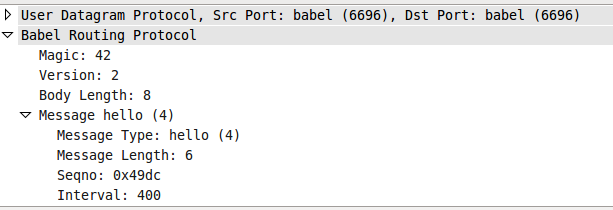
\includegraphics[width=\textwidth]{img/babel_hello}
        \caption{Babel Hello}
        \label{img:testAufbau}
	\end{figure}	
	Mit der \verb!Hello! Message teilt ein Router seinen Nachbarn mit das er existiert.	
	
	\subsubsection{ihu}
	\begin{figure}[H]
        \centering
                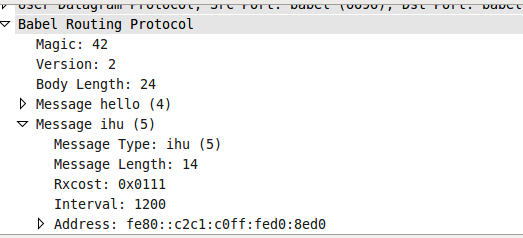
\includegraphics[width=\textwidth]{img/babel_ihu}
        \caption{Babel I hear U}
        \label{img:testAufbau}
	\end{figure}
	Die \verb!I hear U! Message ist die Antwort auf eine \verb!Hello! message, sie teilt dem Sender der \verb!Hello! Message mit das er einen Nachbarn hat, welche Adresse dieser benutzt und was die \verb!rxcost! des links die verwendet werden kann um schlecht sichtbare Hosts vom Routing auszuschließen, bzw. stärkere Links zu bevorzugen.
	
	\subsubsection{update}	
	\begin{figure}[H]
        \centering
                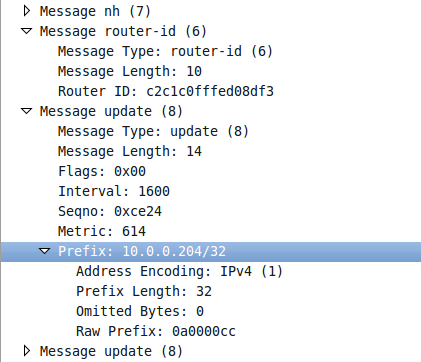
\includegraphics[width=\textwidth]{img/babel_update}
        \caption{Babel Update}
        \label{img:testAufbau}
	\end{figure}
	Eine \verb!Update! Nachricht wird versendet wenn ein Router ein update in seiner Routing Table festgestellt hat um diese zu verbreiten. Das update beinhaltet als primäre Nutzdaten die Metric der Route sowie ihr Ziel (\verb!Prefix!)
	 
	\subsection{OLSR}

\section{Babel}
	\subsection{Experiment 1}\label{sec:babel_experiment1}
	Bei diesem Experiment wurden 10 MB mittels IPerf  unter Verwendung von UDP zwischen 2 Hosts ausgetauscht. Dabei wurde der Traffic über 3 Router geleitet (110-204-104) und UDP als Protokoll verwandt. Die TX-Power aller Geräte betrug dabei 1. 
Den gemessenen Werten Abbildung \ref{img:babel_iperf_tx1} ist zu entnehmen, dass der Paketverlust bei durchschnittlich 88,13\% liegt und eine durchschnittliche Bandbreite von ~749 Kbits/sec erreicht wird.
Begründet sind diese Werte darin, dass mit TX-Power=1 eine sehr geringe Sendeleistung eingestellt wurde. Eine Erhöhung dieser, führt zu einer Verbesserung der Werte, wie in \ref{sec:babel_experiment3} gezeigt wird.

	\begin{figure}
        \centering
                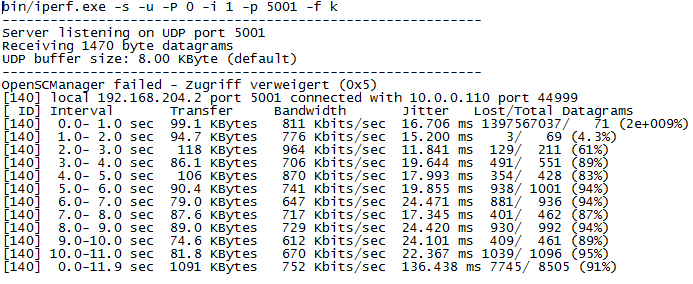
\includegraphics[width=\textwidth]{img/Babel_TX1_Protokoll}
        \caption{IPerf Log mit TX-Power=1}
        \label{img:babel_iperf_tx1}
	\end{figure}
	

	
	\subsection{Experiment 2}
	Bei diesem Versuch sollte das Failoververhalten von Babel getestet werden. Hierzu hat ein Host einen anderen permanent angepingt, um seine Verfügbarkeit zu prüfen. Dabei verlief die Route über alle vier APs. Bei einem Gerät wurde dann die Netzspannung entfernt, um eine Neubildung der Route zu forcieren.
	
	\subsection{Experiment 3}\label{sec:babel_experiment3}
	Dieses Experiment wurde analog zu \ref{sec:babel_experiment1} durchgeführt, allerdings wurde diesmal die TX-Power bei einem der Geräte (110) auf 11 gesetzt, um eine bessere Verbindung herstellen zu können.	

	\begin{figure}
        \centering
                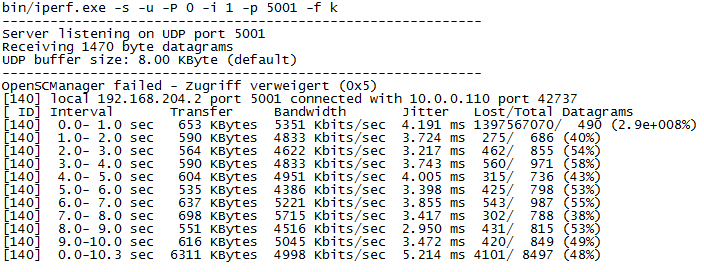
\includegraphics[width=\textwidth]{img/Babel_TX11_Protokoll}
        \caption{IPerf Log mit TX-Power=11}
        \label{img:babel_iperf_tx11}
	\end{figure}
	
Im Kontrast zu \ref{sec:babel_experiment1}, in dem alle Router TX-Power=1 sendeten, ist eine um 38\% Punkte niedrigere Paketverlustrate zu beobachten. Dieser Unterschied von gut einem Drittel resultiert aus der Tatsache, dass zwischen den beiden Routern 110 und 104 eine stärkere Verbindung besteht und auf dieser Strecke weniger Datenpakete verloren gehen.

	\begin{figure}
        \centering
                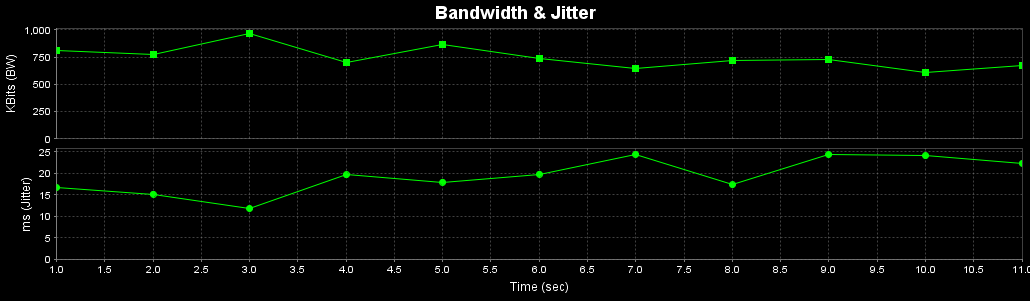
\includegraphics[width=\textwidth]{img/4_UDP_Babel_TX1_10MB}
        \caption{IPerf Log mit TX-Power=11}
        \label{img:babel_iperf_graph_tx11}
	\end{figure}
	
Das Verhalten der Bandbreite und des Jitters ist ähnlich hierzu.
Mit diesem Experiment (in Verbindung mit \ref{sec:babel_experiment3}) konnte gezeigt werden, dass die gesamte Verbindung maßgeblich von der Qualität der einzelnen Verbindungen zwischen den Routern abhängt.

\section{OLRS}
	\subsection{Experiment 1}
	Traffic über 3 Hops	
	
	\subsection{Experiment 2}
	Failover, recovery nach neustart des abgebauten Routers


%\section{Anhang}
	%\subsection{Router Konfigurationen}
		%\lstinputlisting[label=code_110_babel,caption=Babel Konfiguration: Router 110, language=bash]{../Startscripte/110/babeld_start.sh}	
		%\lstinputlisting[label=code_110_olsr,caption=OLSR Konfiguration: Router 110, language=bash]{../Startscripte/110/olsrd_start.sh}	
		%\lstinputlisting[label=code_210_babel,caption=Babel Konfiguration: Router 210, language=bash]{../Startscripte/210/babeld_start.sh}	
		%\lstinputlisting[label=code_210_olsr,caption=OLSR Konfiguration: Router 210, language=bash]{../Startscripte/210/olsrd_start.sh}	
		%\lstinputlisting[label=code_104_babel,caption=Babel Konfiguration: Router 104, language=bash]{../Startscripte/104/babel.sh}	
		%\lstinputlisting[label=code_110_olsr,caption=OLSR Konfiguration: Router 104, language=bash]{../Startscripte/104/olsr.sh}
		%\lstinputlisting[label=code_204_babel,caption=Babel Konfiguration: Router 204, language=bash]{../Startscripte/204/babel.sh}	
		%\lstinputlisting[label=code_210_olsr,caption=OLSR Konfiguration: Router 204, language=bash]{../Startscripte/204/olsr.sh}

\end{document}

